%DIFF 1 new
\documentclass[letterpaper, 10 pt, conference]{ieeeconf}  % Comment this line out if you need a4paper
\IEEEoverridecommandlockouts                              % This command is only needed if
\overrideIEEEmargins                                      % Needed to meet printer requirements.

\usepackage{graphics}    % for pdf, bitmapped graphics files
\usepackage{times}       % assumes new font selection scheme installed
\usepackage{amsmath}     % assumes amsmath package installed
\usepackage{amssymb}     % assumes amsmath package installed
\usepackage{graphicx}
\usepackage{algorithm}
\usepackage[noend]{algpseudocode}
\usepackage[activate=alltext]{microtype}
\usepackage{rotating}
\usepackage{makecell}



\usepackage{subcaption} % enables use multiple figures in a figure
\usepackage{tabu}     % provides advanced tables
\usepackage{booktabs} % enables reference bookstyle tables
\usepackage{xcolor}
\usepackage{import}
\usepackage{url}

% make captions look like original IEEE style
% table:  ieeeconf.cls:2017 \begin{center}{\footnotesize #1}\\{\footnotesize\scshape #2}\end{center}% figure: ieeeconf.cls:
% figure: ieeeconf.cls:2024 \setbox\@tempboxa\hbox{\footnotesize #1.~~ #2}%
\DeclareCaptionFont{ieeetable}{\footnotesize\scshape}
\DeclareCaptionLabelSeparator{ieeefigure}{.~~ }
\DeclareCaptionLabelSeparator{ieeetable}{\\[0.5em]}
\captionsetup[figure]{labelseparator=ieeefigure, font=footnotesize}
\captionsetup[table]{justification=centering, labelseparator=ieeetable, textfont=ieeetable, labelfont=footnotesize}
\captionsetup[subfigure]{font=footnotesize}
\captionsetup{subrefformat=parens}

%% Aligns the last page but causes errors on some machines (such as OSX), so don't use it for now.
\usepackage{flushend}

%% Style hacks to save space
%\setlength{\textfloatsep}{1.3em}
%\setlength{\dbltextfloatsep}{1.3em}
\usepackage[font=small]{caption}

%% Key definitions for text elements. USE THEM
\def\secref#1{Sec.~\ref{#1}}
\def\figref#1{Fig.~\ref{#1}}
\def\tabref#1{Tab.~\ref{#1}}
\def\eqref#1{Eq.~(\ref{#1})}
\def\algref#1{Alg.~\ref{#1}}

%% Other useful macros
\newcommand\todo[1]{\textbf{[TODO: #1}]}
\newcommand\etal{\emph{et~al.}}


%% Some math definition
\def\argmax{\mathop{\rm argmax}}
\def\argmin{\mathop{\rm argmin}}
\newcommand{\bigO}[1]{$\mathcal{O}(#1)$}

%DIFF 2
%%%%%%%%%%%%%%%%%%%%%%%%%%%%%%%%%%%%%%%%%%%%%%%%%%%%%%%%%%%%%%%%%%%%%%%%%%%%%%%%

\title{\LARGE \bf Gradient and Log-based Active Learning\\ for Semantic Segmentation of Crop and Weed for Agricultural Robots}

\author{Rasha Sheikh \and Andres Milioto \and Philipp Lottes \and Cyrill Stachniss \and Maren Bennewitz \and Thomas Schultz% <-this % stops a space
  \thanks{All authors are with the University of
    Bonn, Germany. This work has partly been supported by the German Research Foundation under Germany's Excellence Strategy, EXC-2070 - 390732324 (PhenoRob).}%
}

\begin{document}
\maketitle
\thispagestyle{empty} 
\pagestyle{empty}


%%%%%%%%%%%%%%%%%%%%%%%%%%%%%%%%%%%%%%%%%%%%%%%%%%%%%%%%%%%%%%%%%%%%%%%%%%%%%%%%
\begin{abstract}
Annotated datasets are essential for supervised learning. However, annotating
large datasets to  train deep neural networks that perform well is a tedious
and time-intensive task. This paper  addresses active learning in the context
of semantic segmentation with the goal of reducing the  human labeling effort.
Our application is agricultural robotics  and we focus on the task of
distinguishing between crop and weed plants from image data. A key challenge in this
application is the  transfer of an existing semantic segmentation CNN to a new
field, in which growth stage, weeds, soil, and weather condistion differ. 
We propose a novel approach that, given a trained model on one field together with 
rough foreground/background segmentation,
refines the network on a substantially different field  providing an effective
method of selecting samples to annotate for supporting the transfer. Two of our ranking approaches take
 into account the influence of the so far unlabeled samples on the
weights of the network and select them accordingly for annotation. The other ranking approaches 
use the loss and uncertainty measures provided by the network then ranks samples on a log-scale to ensure diversity.
We evaluated our approach on two challenging  datasets from the agricultural
robotics domain and show that we achieve a higher accuracy with a  smaller
number of samples compared to randomly selecting samples for annotation, which consequently reduces the required human labeling  effort.

\end{abstract} 

%%%%%%%%%%%%%%%%%%%%%%%%%%%%%%%%%%%%%%%%%%%%%%%%%%%%%%%%%%%%%%%%%%%%%%%%%%%%%%%%
\section{INTRODUCTION}
\label{sec:intro}

The ability to  interpret the scene in front of a robot is key for
intelligent behavior in several applications. For example, precision farming
robots need to know which type of plant they perceive or autonomous cars need to
know  which object in their surroundings is a car, a pedestrian, or a
cyclist. These  classification or semantic segmentation tasks are typically
tackled using  convolutional neural networks~(CNNs) operating on  image data.
In order to perform  well, neural networks need to be trained with
appropriately annotated datasets.

The performance of most supervised learning approaches and especially deep
learning  systems is related to the quality and quantity of training data.
Annotated training data, however, has a high cost as often a larger number of
labeled training data is  required.  In this work, we focus on optimizing the
training set generation for  semantic segmentation of image data obtained
from a mobile robot. Semantic segmentation refers to the task of computing a
pixel-wise  labeling of the images. More concretely, we address the
agricultural robotics  application in which robots should perform automated
weed control. For the semantic  segmentation, this means that we need to
compute the semantic label ``crop'', ``weed'',  or ``misc'' for each pixel in
the image. This task is particularly challenging  as the field conditions
often change substantially between years, regions, weather, and  soil
conditions as can be seen in Figure~\ref{fig:datasets_images}.  

One solution to adapt and refine existing semantic
segmentation systems to new field conditions  is through additional labeled data from the
new field. As these new annotations need to be executed at the end-users site,
one is interested in keeping this effort as low as possible. 
%Therefore, this task
% is a perfect domain for active  learning approaches that try to reduce
%the required amount of data to be annotated.
%
Given annotated data on one agricultural field and a CNN that was trained
on it, we address the problem of transferring this knowledge to new fields with
minimum effort.  Datasets from different fields reveal different crop and weed
statistics. They often differ by soil type, weather condition, or
various small objects that can be found  on the ground, such as stones, dried
vegetation, or marks from agricultural machines, i.e., patterns that are
neither crop nor weed. Additionally, the robot can acquire  images of plants
at a certain growth stage in one field, while the growth state on the  target
field is different. Lastly, artifacts such as contrast changes can be found in
the camera images captured from the various locations.  As illustrated by 
Lottes \etal~\cite{lottes2018ral,lottes2017iros}, these conditions make
it difficult to simply reuse a previously trained network from one  field and
infer the labels on another. 
%Thus, 
%the network has to be
%re-trained on  annotated images taken in the new field. We propose an
%active learning  approach to select samples that the network will most benefit
%from and will generalize  to the rest of the unlabeled data while minimizing
%the effort of annotating images.


    \begin{figure}
    \centering
    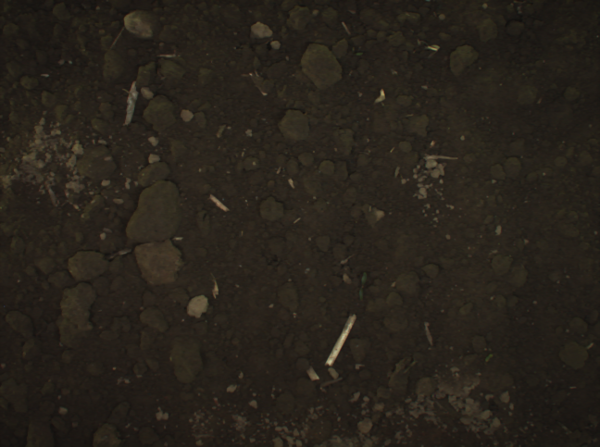
\includegraphics[width=0.32\linewidth]{pics/bonn/images/bonirob_2016-04-28-12-20-29_6_frame217.png}
    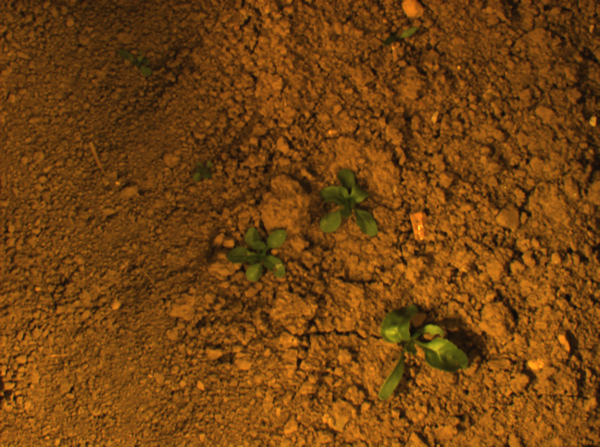
\includegraphics[width=0.32\linewidth]{pics/stuttgart/images/masks_8mm_fromImages_frame479.png}
    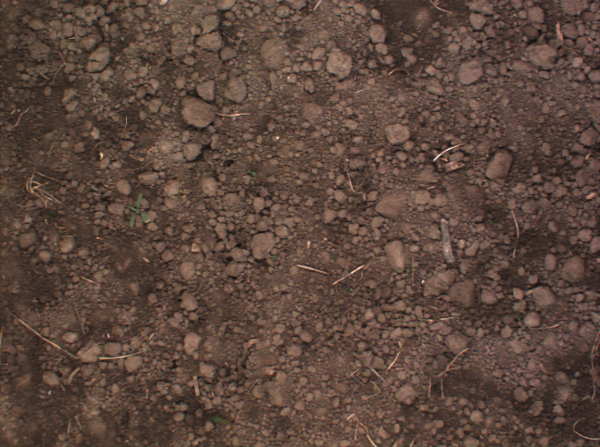
\includegraphics[width=0.32\linewidth]{pics/zurich/images/bonirob_2016-10-13-09-03-00_0_frame66.png}\\[1mm]
    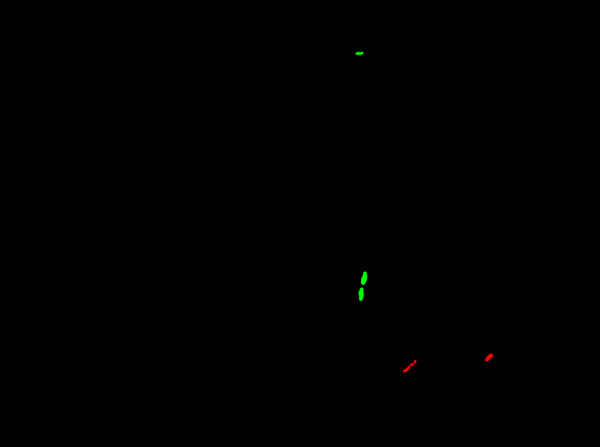
\includegraphics[width=0.32\linewidth]{pics/bonn/annotations/bonirob_2016-04-28-12-20-29_6_frame217.png}
    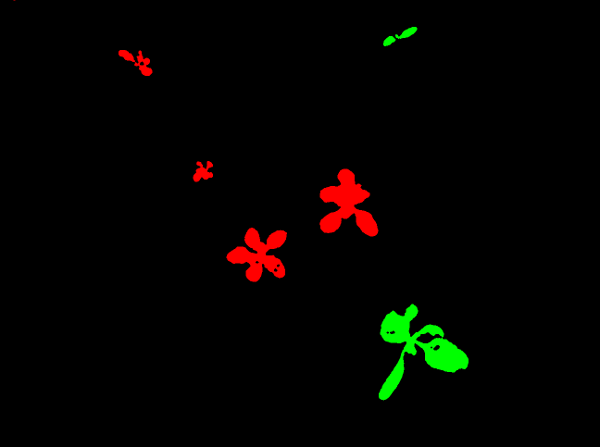
\includegraphics[width=0.32\linewidth]{pics/stuttgart/annotations/masks_8mm_fromImages_frame479_GroundTruth_iMap.png}
    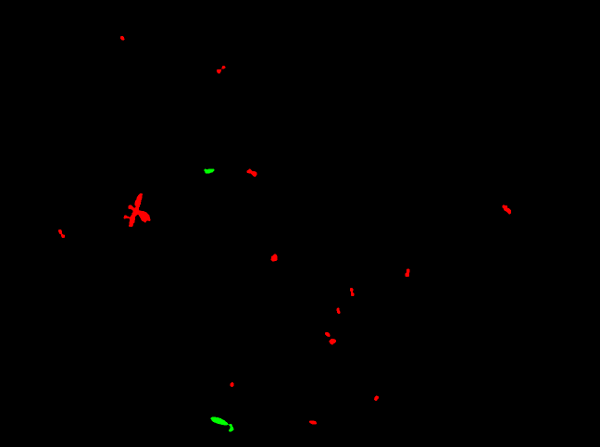
\includegraphics[width=0.32\linewidth]{pics/zurich/annotations/bonirob_2016-10-13-09-03-00_0_frame66.png}
    \caption{Sample images from the Bonn, Stuttgart, and Zurich
      sugar beet datasets in the first, second, and third column,
      respectively. The first row shows the RGB images and the second
      row shows their annotations~(green denotes crop while red
      denotes weed). As can be seen, the appearance differs
      substantially.}
    \label{fig:datasets_images}
\end{figure}

The main contribution of this work is a new active learning strategy that
intelligently pick images taken under new conditions to re-train an existing network.
We start by picking samples based 
on the uncertainty of their predictions, and separately on the network loss with respect 
to pseudo labels. We add diversity to the sample selection using a log-space ranking.
Moreover, we look into the effect training samples will have on the weight gradients of the CNN,
and pick samples accordingly.
Our strategy is based  on the observation that given a trained model and unseen
samples from  a different domain, the samples that the network performs most
poorly on, especially at the  beginning, will have the largest weight
gradients and consequently the largest impact on the  weights. This strategy might appear to be circular, since computing gradients already requires class labels at a stage where are still selecting images for labeling.  We circumvent this by using pseudo ground truth that we obtain with very weakly supervised segmentation. Our approach
selects samples in batches, each time refining the network, then computing a
new  ranking of the unlabeled data. The best samples are then selected and the
network is re-trained. To compute the real gradients, corresponding ground
truth data is needed. Thus, in our approach, we approximate the ground truth as the result of unsupervised segmentation to estimate the gradient.  We
evaluated our framework using three distinctive sugar beet datasets~\cite{chebrolu2017agricultural} that have different characteristics.  Our results indicate that our method produces a
higher accuracy on the datasets with a fewer  number of samples compared to
random sampling for annotation.


 
   
   %  \begin{figure*}
   %  \vspace{1em}
   %  \centering
   %  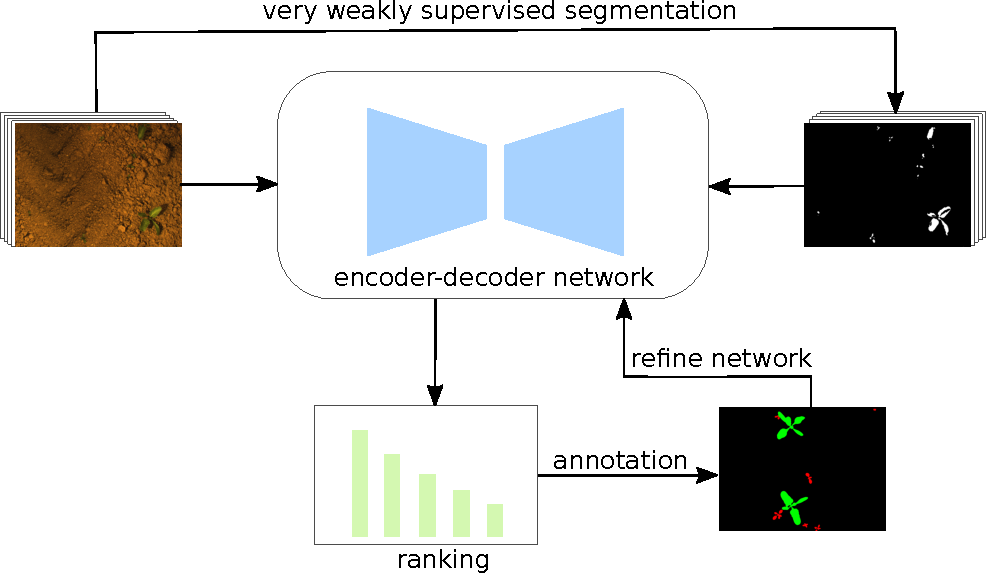
\includegraphics[scale=0.8]{pics/output_system_overview.pdf}
   %    \caption{Overview figure of our system. We first perform very weakly supervised segmentation to obtain pseudo ground truth. Given the labels and different measures produced by the network, we rank the unlabeled samples and pick them accordingly for annotation. These are then used to refine the entire network.}
   %  \label{fig:overview}        
   % \end{figure*}


   

%%%%%%%%%%%%%%%%%%%%%%%%%%%%%%%%%%%%%%%%%%%%%%%%%%%%%%%%%%%%%%%%%%%%%%%%%%%%%%%%
\section{RELATED WORK}
\label{sec:related}



Several works focusing on the elimination or reduction of herbicide use,
through the incorporation of autonomous ground robots in crop fields, have
been introduced to the community in the last years~\cite{ducket2018arxiv,liebisch2016wslw,mccool2018ral}.
A key component of each of these unmanned platforms is a core perception system that
has the ability to accurately distinguish crops from weeds in order to effectively
and selectively apply the desired individual treatment~\cite{lottes2018iros, mccool2017ral,milioto2017uavg,milioto2018real,sa2018rs}.
These systems allow autonomous robots to perform actuation in the fields without human supervision, treating each plant individually.
All of the works referenced, however, are based on supervised learning approaches which take large amounts of pixel-accurate hand-labeled images for training. 

Accordingly, one of the main bottlenecks of these visual processing pipelines is the amount of expensive labeled training data required to deploy them in real agricultural fields, which often limits their applicability. In order to tackle this data starvation problem, we propose an active learning based solution.

Numerous works on general active learning have been presented in the community~\cite{settles2009active,guyon2011results,holub2008entropy, yoo2019learning}. The most common measures for selecting samples are based on the uncertainty of the network~\cite{zhou2017fine, yang2017suggestive, gal2017deep, wang2017cost} and diversity~\cite{zhou2017fine, dutt2016active, kading2016active}.  Sener \etal~\cite{sener2017geometric} assert based on the experiments they performed that uncertainty based approaches are not effective for active learning with CNNs. They hypothesize that this is not due to the inaccurate estimate of uncertainty by the network, rather to the ineffectiveness of uncertainty based approaches to cover the space of image features.

The Expected Model Output Change Principle (EMOC) developed by Freytag \etal~\cite{freytag2014selecting} tries to avoid selecting samples that are redundant and K{\"a}ding \etal~\cite{kading2016active} follow this approach with deep neural networks. This principle measures how a model would perform with and without the candidate sample. Given that the labels are unknown, a marginalization over the possible labels is needed. This marginalization however can be expensive when having a large number of classes, so the authors use maximum a-posteriori approximation instead and use the class with the highest probability prediction.

Uncertainty estimation for active learning can be performed using Monte-Carlo dropout as in~\cite{gal2017deep} or with an ensemble of deep networks. Beluch \etal~\cite{beluch2018power} compare both of these approaches on different datasets. They found that an ensemble of deep classifiers has a superior performance even with a smaller number of models. They conclude that Monte-Carlo dropout approaches suffer from a lower diversity and a smaller model capacity.

The works mentioned previously and the current state-of-the-art methods for active learning including~\cite{gal2017deep,beluch2018power,sener2017active,yoo2019learning} are either more suitable for tasks other than pixel-wise semantic segmentation of images with CNNs and/or are memory and computationally expensive.

Weakly supervised segmentation is an active research topic~\cite{wei2018revisiting, acuna2018efficient, tang2018normalized, kwak2017weakly}. In the context of self-learning, Zhang \etal~\cite{zhang2018self} use labels obtained with K-means graph cuts as ground truth for their network. The predictions produced by the model are then used as the target labels for the next iteration of the process.  

Different to the previously mentioned works, we experiment with approaches that directly measure how annotated samples can affect the gradients. We use labels obtained with very weak supervision as pseudo ground truth and compute the gradients w.r.t the weights. We then refine a pre-trained network with the newly annotated samples in an iterative manner. 

Our intuition for using gradients is driven by the observation that the greater the mismatch is between the predicted segmentation and the ground truth, the larger the change is to the weights. This is in contrast to most of the approaches mentioned earlier that rely on the confidence of the network which may not be the best indication of the best samples to choose for annotation, as the network output might actually be correct although the network is uncertain about it.

Previous work, such as the Expected Gradient Length (EGL)~\cite{huang2016active, settles2008multiple}, has explored how changes in model parameters can be exploited for sample selection. However, it computes the expectation of the gradient norm over all possible annotations, which would be prohibitively expensive for pixel-wise semantic segmentation of images. We instead compute gradients from rough foreground/background segmentation.

Du \etal~\cite{du2018adapting} use gradient similarity to determine when an auxiliary task is helpful for transfer learning to the main task and when it can be hurtful. Although in our work, the weakly supervised setting can be seen as an auxiliary task, we only use the gradients computed there as a guidance to choose samples for annotations. These gradients are not used to measure similarity with those of the main task nor are the parameters of the main task updated with those gradients. 


%Several works focusing on the elimination or reduction of herbicide use,
%through the incorporation of autonomous ground robots in crop fields, have
%been introduced to the community in the last years~\cite{ducket2018arxiv, liebisch2016wslw, mccool2018ral}.
%A key component of each of these unmanned platforms is a core perception system that
%has the ability to accurately distinguish crops from weeds in order to effectively
%and selectively apply the desired individual treatment~\cite{ lottes2018iros, mccool2017ral,milioto2017uavg,milioto2018real, sa2018rs}.
%These systems allow autonomous robots to perform actuation in the fields without human supervision, treating each plant individually.
%All of the works referenced, however, are based on supervised learning approaches which take large amounts of pixel-accurate hand-labeled images for training. 
%Accordingly, one of the main bottlenecks of these visual processing pipelines is the amount of expensive labeled training data required to deploy them in real agricultural fields, which often limits their applicability.
%
%In order to tackle this data starvation problem, we propose an active learning based solution. Numerous works on general active learning have been presented in the community~\cite{settles2009active,guyon2011results,holub2008entropy}. Recently, the research topic of using active learning in combination with deep learning has received attention. We focus in this section on the different approaches that explored active learning within a deep learning framework.
%
%Settles~\cite{zhou2017fine} defines measures of entropy and diversity to select new samples for annotation. The entropy of a patch is calculated based on the classification uncertainty of the network, whereas the diversity is computed using the Kullback Leibler divergence of different patches within the same sample candidate. A pre-trained network is then refined using the samples with the highest entropy and diversity.
%
%Yang \etal~\cite{yang2017suggestive} select samples that the network is uncertain of and that are representative of other images in the dataset. The uncertainty is measured by bootstrapping, where multiple fully convolutional networks (FCNs) are trained, and the variance among  these trained models is used to estimate the uncertainty. In order to choose samples that are highly similar to others in the training set, features are extracted from the encoding part of the network, and the cosine similarity between pairs of images is calculated. 
%
%Dutt Jain \etal~\cite{dutt2016active} create foreground masks in an iterative manner. Samples that are deemed most valuable for annotation are selected. Their ground truth annotation is then propagated to new samples and the process is repeated. To pick samples for which human annotation will propagate well, the authors build a Markov Random Field (MRF) joint segmentation graph. The graph is then used to find samples that have the largest influence, diversity and uncertainty. The influence and diversity are computed using the cosine-similarity of different images features, while the uncertainty is estimated using a regressor that quantifies the quality of a prediction. 
%
%Gal \etal~\cite{gal2017deep} evaluate different acquisition functions. An active learning system would use such an acquisition function to choose the best next sample to annotate. These functions include maximizing the predictive entropy of a model given the training set and a new sample, and closely related to that is the variation ratio measure. Another function maximizes the mutual information between predictions and the model posterior. These different measures are compared using a Bayesian Convolutional Neural Network that has a prior probability distribution over the model parameters.  
%
%Uncertainty estimation for active learning can be performed using Monte-Carlo dropout as in~\cite{gal2017deep} or with an ensemble of deep networks. These uncertainties can then be used in the different acquisition functions described earlier. Beluch \etal~\cite{beluch2018power} compare both of these approaches on different datasets. They found that an ensemble of deep classifiers has a superior performance even with a smaller number of models. They conclude that Monte-Carlo dropout approaches suffer from a lower diversity and a smaller model capacity.
%
%Sener \etal~\cite{sener2017geometric} assert based on the experiments they performed that uncertainty based approaches are not effective for active learning with CNNs. They hypothesize that this is not due to the inaccurate estimate of uncertainty by the network, rather by the ineffectiveness of uncertainty based approaches to cover the space of image features. They instead propose to choose samples such that the largest distance between a new sample and its closest neighbor in the selected subset is minimized.
%
%Wang \etal~\cite{wang2017cost} select two sets of samples for annotation that can then be used by the network to refine the model. The first set consists of samples that the network is uncertain about. These include samples with the lowest softmax confidence values, samples with the highest entropy, and lastly samples with a small margin of probability difference between the most probable class and the second most probable class. This first set is then presented to a human for annotation. The second set consists of samples that the network is highly certain about, these are assigned their predicted classes as pseudo labels and added to the set of training samples without asking a human to annotate them.
%
%The Expected Model Output Change Principle (EMOC) developed by Freytag \etal~\cite{freytag2014selecting} tries to avoid selecting samples that are redundant and K{\"a}ding \etal~\cite{kading2016active} follow this approach with deep neural networks. This principle measures how a model would perform with and without the candidate sample. Given that the labels are unknown, a marginalization over the possible labels is needed. This marginalization however can be expensive when having a large number of classes, so the authors use maximum a-posteriori approximation instead and use the class with the highest probability prediction.
%
%In the context of self-learning, Zhang \etal~\cite{zhang2018self} use labels obtained with K-means graph cuts as ground truth for their network. The predictions produced by the model are then used as the target labels for the next iteration of the process.  
%
%Du \etal~\cite{du2018adapting} use gradient similarity to determine when an auxiliary task is helpful for transfer learning to the main task and when it can be hurtful. Although in our work, the weakly supervised setting can be seen as an auxiliary task, we only use the gradients computed there as a guidance to choose samples for annotations. These gradients are not used to measure similarity with those of the main task nor are the parameters of the main task updated with those gradients.  
%
%Several works have explored weakly supervised segmentation. By having convolution kernels with different dilation rates, Wei \etal~\cite{wei2018revisiting} are able to improve object localization in weakly and semi supervised settings. Acuna \etal~\cite{acuna2018efficient} use reinforcement learning to train an encoder and RNN decoder model that is able to predict polygon vertices of an object. Tang \etal~\cite{tang2018normalized} combine partial cross entropy loss for labeled pixels with normalized cut loss. Kwak \etal~\cite{kwak2017weakly} define a superpixel pooling layer that performs average pooling on upsampled feature maps using superpixels as the pooling layout.
%
%Different to these works, we experiment with approaches that directly measure how annotated samples can affect the gradients. We use labels obtained with very weak supervision as pseudo ground truth and compute the gradients w.r.t the weights. We then refine a pre-trained network with the newly annotated samples in an iterative manner. Our intuition is driven by the observation that the greater the mismatch is between the predicted segmentation and the ground truth, the larger the change is to the weights. This is in contrast to most of the approaches mentioned earlier that rely on the confidence of the network which may not be the best indication of the best samples to choose for annotation, as the network output might actually be correct although the network is uncertain about it.
%
%Previous work, such as the Expected Gradient Length (EGL)~\cite{huang2016active, settles2008multiple}, has explored how changes in model parameters can be exploited for sample selection. However, differently it computes the expectation of the gradient norm over all possible annotations, which would be prohibitively expensive for pixel-wise semantic segmentation of images. We instead compute gradients from rough foreground/background segmentation.


    \begin{figure}
    \centering
    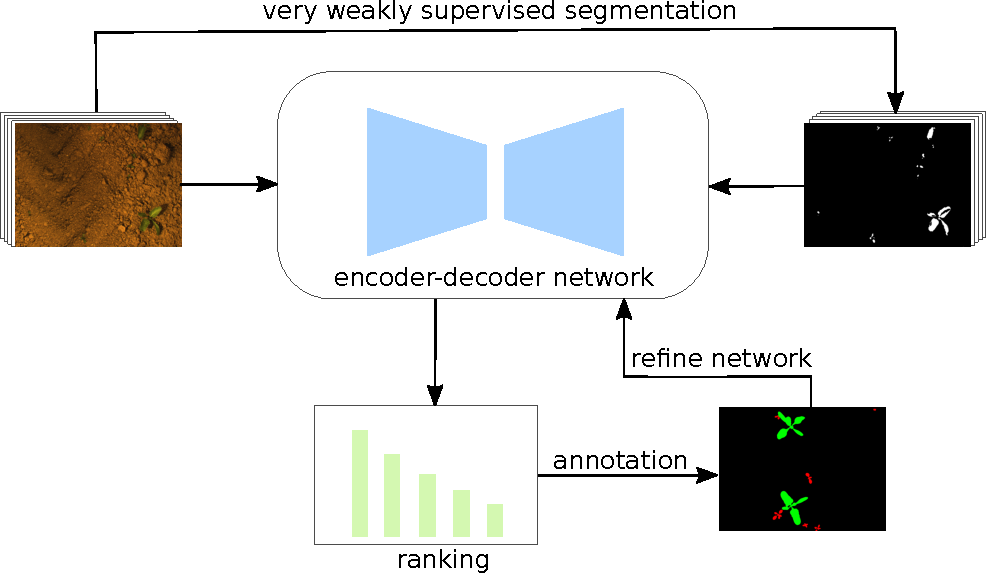
\includegraphics[width=\linewidth]{pics/output_system_overview.pdf}
      \caption{Overview of our approach. The key idea is that we first
        perform a very weakly supervised segmentation to obtain pseudo
        ground truth. Given the labels and different ranking measures
        obtained from the network, we rank the unlabeled samples and pick them
        accordingly for annotation. Those samples are then used to refine the entire network.}
    \label{fig:overview}        
   \end{figure}


\section{Our Approach to Effective Sample Selection}
\label{sec:approach}

Figure~\ref{fig:overview} shows an overview of our framework.
The key idea of our approach is to perform a very weakly supervised segmentation to obtain pseudo ground truth. Given the labels and different measures produced by the network, we rank the unlabeled samples and pick them accordingly for annotation. These are then used to refine the entire network.


Our CNN for semantic segmentation relies on Bonnet~\cite{milioto2018bonnet}.
The used network is based on SegNet~\cite{badrinarayanan2017segnet} and ENet~\cite{paszke2016enet}. It has an encoder-decoder structure with a total of 25 [5x5] convolutional layers. It uses batch normalization, residual connections, ReLU as the non-linearity layer, and the focal loss function~\cite{DBLP:conf/iccv/LinGGHD17}.
As input to our network, we only use the standard RGB channels of a camera.

In order to perform the semantic segmentation in sugar beet field for agricultural robotics tasks,
we train our model on the Bonn sugar beet dataset~\cite{chebrolu2017agricultural}. We then refine the trained model on other datasets by incrementally selecting batches of samples. The datasets differ in their crop/weed statistics and the images acquired with the cameras also differ in their illumination. Therefore, simply running the trained model to segment the vegetation in other fields does not work.

%In this section, we describe four different approaches to sample selection for active learning based on uncertainty (see \secref{ssec:unc}), loss (see \secref{ssec:loss}), and gradients (see \secref{ssec:normgrad} and \secref{ssec:gradproj}).
%Our  sample section strategies are the gradient-based ones.
%We design these novel gradient-based approaches to select samples, one that is based on the norm of the network gradients, and the other on the norm of projected out gradients. We also combine measures already provided by the network, namely uncertainty and loss, with log-scale ranking. 


In this section, we describe four different approaches to sample selection for active learning. We combine measures already provided by the network, namely uncertainty and loss, with log-scale ranking (see \secref{ssec:unc}), loss (see \secref{ssec:loss}). We also design novel gradient-based approaches to select samples, one that is based on the norm of the network gradients, and the other on the norm of projected out gradients (see \secref{ssec:normgrad} and \secref{ssec:gradproj}).



%We design novel gradient based approaches to select samples, one that is based on the norm of the network gradients, and the other on the norm of projected out gradients. In the experiments section we illustrate the performance of these methods and compare them to other approaches, including random selection of samples, selecting samples driven by the training loss, or driven by the uncertainty of the network.
   
%We experimented with different approaches to select samples. The baseline is randomly selecting samples for annotation in batches of 10. The other approaches include selecting samples driven by the training loss, the norm of the network gradients, and the norm of projected out gradients. In the experiment section we also show how the model performs when sample selection is guided by the uncertainty of the network.

% this is repeated in the following subsection:
%% we thought we would add it again early on because one of the reviewers was confused by the meaning of pseudo ground truth

To compute the strategies explained in the following subsections, we use what we refer to in the text as pseudo ground truth. These are foreground masks generated by clustering with very weak supervision as detailed in the subsequent section. An example is shown in Figure~\ref{fig:unsupervised_foreground}.

\begin{figure}
    \centering
    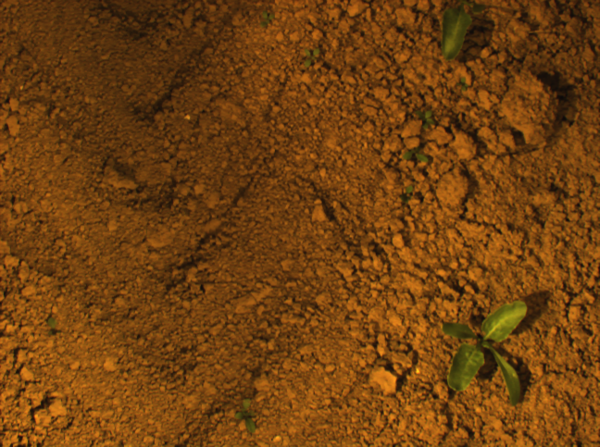
\includegraphics[width=0.32\linewidth]{pics/unsupervised/img_masks_8mm_fromImages_frame256.png}
    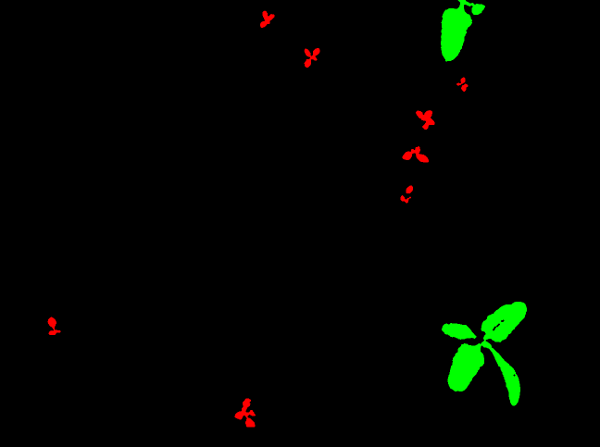
\includegraphics[width=0.32\linewidth]{pics/unsupervised/gt_masks_8mm_fromImages_frame256_GroundTruth_iMap.png}
    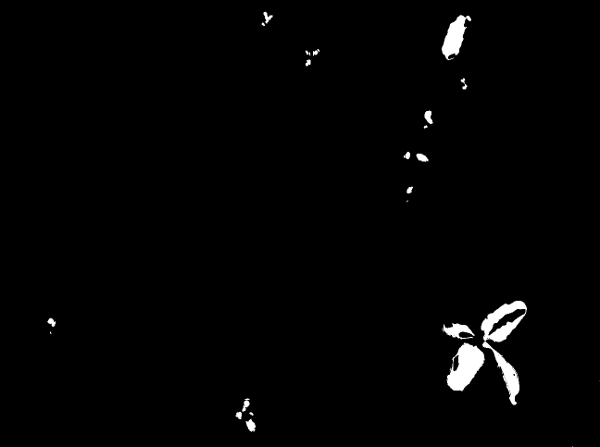
\includegraphics[width=0.32\linewidth]{pics/unsupervised/lbl_masks_8mm_fromImages_frame256.png}
    \caption{Very weakly supervised segmentation used as pseudo ground
      truth by our approach.  Left: Input image. Middle: Ground truth semantic
      segmentation; Right: Foreground segmentation of vegetation
      provided by k-means clustering. Note that only such a rough
      segmentation as pseudo ground truth is enough for our approach.}
    \label{fig:unsupervised_foreground}
\end{figure}


%rough and easy to compute segmentation is sufficient for the purpose of selecting images for annotation

%\subsection{Uncertainty}
%
%To infer the pixel-wise semantic segmentation of a new image, the network computes softmax probabilities in its last layer. The probabilities can serve as a guide as to which samples the network is most uncertain of. For every image passed through the network, we compute the following measure of the prediction confidence:
%\begin{align}
%u(\bold{x}) &= \frac{1}{N} \sum_{i=1}^N \max_c p(c  \mid  x_i),
%\end{align}  
%
%where $x_i$ is pixel $i$ in image $\bold{x}$, $c$ is the predicted class and $N$ is the number of pixels in the image.
%
%We then sort the images based on the computed uncertainty measure in a descending order and pick the images accordingly to refine the network on a new dataset. The images are selected on a log-space scale, rather than selecting those with the highest uncertainty, as we found out that the network learns better when presented with diverse samples.
%
%We generate a string of numbers, starting from zero, that are spaced evenly on a log scale. These numbers are then used as the indices of the samples to be selected. Since the samples are sorted, this approach would more heavily select samples that have higher uncertainty values while not completely discarding those that the network is more confident of their predictions. 
%
%The log-space approach is used in the following methods as well.


\subsection{Setup}

We evaluate our different approaches by first training a network on the Bonn sugar beet dataset then refining it on the Stuttgart and Zurich datasets separately. To refine the network we pick unlabeled samples in batches of 10 using one of the methods described in this section. Once the samples are annotated, they are given to the network. We repeat this process iteratively, each time refining the network on all of the newly annotated samples. 

%For the methods presented in sections \ref{sec:loss}, \ref{sec:grad_norm}, and \ref{sec:grad_proj}, we first obtain foreground masks with very weak supervision. 


\subsection{Foreground Masks}

We first obtain foreground-background segmentation masks by clustering the values of the RGB channels. We run k-means to determine 20 cluster representatives from 10 randomly selected images. After viewing a single image that contains all 20 clusters, a human annotator chooses which clusters represent vegetation. In our experiments, it was enough to select two clusters. Therefore, the human annotation effort is merely a few seconds for one dataset. In accordance with previously used terminology \cite{zhang2018self}, we refer to this step as being very weakly supervised, since it only involves inspecting a single image. Figure~\ref{fig:unsupervised_foreground} shows an image, its ground truth and the foreground segmentation (pseudo ground truth) provided by clustering. It is an important finding from our experiments that a rough and easy to compute segmentation is sufficient for the purpose of selecting images for annotation. This makes our proposed gradient-based approach feasible in practice.



\subsection{Sample Selection Using Uncertainty}
\label{ssec:unc}
To infer the pixel-wise semantic segmentation of a new image, the network computes softmax probabilities in its last layer. The probabilities can serve as a guide as to which samples the network is most uncertain of. For every image passed through the network, we compute the following measure of the prediction confidence:
\begin{align}
u(\bold{x}) &= \frac{1}{N} \sum_{i=1}^N \max_c p(c  \mid  x_i),
\end{align}  
\noindent
where $x_i$ is pixel $i$ in image $\bold{x}$, $c$ is the predicted class and $N$ is the number of pixels in the image.

We then sort the images based on the computed uncertainty measure in a descending order and pick the images accordingly to refine the network on a new dataset. We found that it is helpful for the network to have diverse samples, especially because our goal is to train using only few annotated images. We therefore rank the samples on a log-space scale as follows: We generate a string of numbers, starting from zero, that are spaced evenly on a log scale. These numbers are then used as the indices of the samples to be selected. Since the samples are sorted, this approach would more heavily select those that have higher uncertainty values while not completely discarding images that the network is more confident of.



\subsection{Sample Selection Using Loss} \label{sec:loss}
\label{ssec:loss}

The loss of the network is an indication of the segmentation error. Given that training neural networks with backpropagation is driven by the loss, it also provides a useful cue as to which samples the network will most benefit from. We compute the focal loss \cite{DBLP:conf/iccv/LinGGHD17} based on the pseudo ground truth.

The images are sorted based on this loss in a descending order and selected on a log-scale ranking to encourage diversity as explained earlier.

% consisting of a foreground-background segmentation that we achieve using k-means clustering on the RGB channels.

%Initially, we use k-means to determine 20 cluster representatives from 10 randomly selected images. After viewing a single image that contains all 20 clusters, a human annotator chooses which clusters represent vegetation. In our experiments, it was enough to select two clusters. Therefore, the human annotation effort is merely a few seconds for one dataset. In accordance with previously used terminology \cite{zhang2018self}, we refer to this step as being very weakly supervised, since it only involves inspecting a single image. 

%Pseudo ground truth is generated for all unlabeled images by assigning pixels to the selected clusters, and the loss is computed with respect to it. 

%The images are sorted based on this loss in a descending order. Rather than selecting those with the highest loss, we found that the network learns better when presented with diverse samples. The samples are therefore selected on a log-scale space.
%
%We generate a string of numbers, starting from zero, that are spaced evenly on a log scale. These numbers are then used as the indices of the samples to be selected. Since the samples are sorted, this approach would more heavily select those that have higher loss values while not completely discarding images that the network is performing well on.

Note that the pseudo ground truth is only used to compute the loss but the network weights remain unchanged and are only later updated with the manual annotations of the selected samples.


\subsection{Sample Selection Using Norm of Gradients} \label{sec:grad_norm}
\label{ssec:normgrad}

For this approach and the following one, we pick those samples for annotation that might have the largest impact on the network weights. The norm of the network gradients is a measure that is indicative of which samples will affect the weights more than others. Although the loss and norm of gradients are correlated, there are instances where the loss could be high for certain samples, yet the gradient is locally small. This depends on the loss function and the state of the current network parameters. 

As in the previous approach, we use labels from very weakly supervised segmentation as pseudo ground truth. We run the network on the training images for one epoch (to maintain computational efficiency) and compute the gradients. Again we note that this step is only used to compute the gradients but the network weights remain unchanged. Once we have the gradients, we compute the $L_2$ norm of those in the last two layers of the network (the classifier layer and the one immediately before it):
\begin{align}
n_g(\bold{x}) &=  \left\lVert \nabla_{w_f} \mathcal{L}(\bold{x}) \right\rVert,
\end{align}  
where $\bold{x}$ is the image and $w$ are the weights of the final two layers.

The images are sorted based on this measure in a descending order and again we pick samples on a log-space scale afterwards as explained earlier.

\subsection{Sample Selection Using Gradient Projection} \label{sec:grad_proj}
\label{ssec:gradproj}

The log-space in the previous approaches was used to ensure there is enough diversity among the samples so that the network does not overfit on them and can generalize to unseen data. Here we use a different method that relies on the space spanned by the gradients where we project onto the orthogonal complement of the gradients of the selected samples. For every picked, sample we project the gradients of all remaining samples onto the selected sample gradient. We then subtract the projected gradient from the original gradients. The residual we are left with indicates which samples have the strongest remaining effect on the weights after accounting for the already selected samples. This can be formulated as:
\begin{align}
n_p(\bold{x}) &=  \left\lVert \bold{g_x} - \sum_{i=1}^S \frac{\left\langle \bold{g_i}, \bold{g_x} \right\rangle}{\left\langle \bold{g_i}, \bold{g_i} \right\rangle} \bold{g_i} \right\rVert,
\end{align}
where $\bold{x}$ is the image, $\bold{g_i}$ is the gradient of the $i$th sample out of $S$ previously selected samples, and $\bold{g_x}$ is the gradient of the current sample.

We select samples one by one, each time sorting them according to this measure and choosing the one with the highest norm of the residual. To pick the first sample, we choose that with the highest norm of the gradient.



%%%%%%%%%%%%%%%%%%%%%%%%%%%%%%%%%%%%%%%%%%%%%%%%%%%%%%%%%%%%%%%%%%%%%%%%%%%%%%%%
\section{Experimental Evaluation}
\label{sec:exp}

In this section, we demonstrate the effectiveness of the approaches we designed for active learning and evaluate the performance of the different sample selection methods on different datasets.

\subsection{Datasets}

The datasets we used were acquired with a Bosch Deepfield Robotics UGV in three different fields: Bonn and Stuttgart in Germany, and Zurich in Switzerland. The datasets have weed and crop plants at different stages of growth and Figure~\ref{fig:datasets_images} shows sample images from the different datasets. The images vary in their illumination, soil type, and class statistics, hence the need for transfer learning. The images have been annotated into three classes:  weed, crop, and soil/misc.  Table~\ref{tab:datasets_stats} shows the number of images in each dataset and the ratio of foreground pixels. It can be clearly seen that there is a high imbalance of classes in the data.



    \begin{table}
       \vspace{1em}
        \centering
        \caption{Datasets Statistics of Crop and Weed Plants}
        \begin{tabular}{@{}lccccc@{}} 
            \toprule
              & Bonn & Stuttgart & Zurich \\ 
            \midrule 
    		  Images  & 8230 & 2584 & 2577 \\ \addlinespace
    		  Crop pixels & 2.0\% & 1.5\% & 0.4\%  \\ \addlinespace
    		  Weed pixels & 0.3\% & 0.7\% & 0.1\%  \\    
            \bottomrule
        \end{tabular}
        \label{tab:datasets_stats}
    %       \vspace{10em}
    \end{table}
     


We follow the approach of \cite{milioto2018real} and split the new dataset into three sets: 40\% for training, 10\% for validation, and 50\% for testing. The samples are picked from the training set. All experiments were conducted on four Nvidia Titan~X GPUs.  


\subsection{Re-Training Performance}

The experiments in this section are designed to show how the proposed sample selection strategies impact the performance of the network in the new environment. For quantifying the performance, we use the mean Intersection over Union (mIoU) as the performance measure. To provide the lower and upper bounds for the methods, we list in Table~\ref{tab:null_and_fully_supervised}  the mIoU for each dataset when running the model without any refinement as well as when training on all of the samples. 

            \begin{table}
          \vspace{1em}
        \centering
        \caption{IoU without any refinement (lower bound) and IoU when training on the whole dataset (upper bound).}
        \begin{tabular}{@{}lcc@{}} 
            \toprule
              &  No Refinement  & Fully supervised \\ 
            \midrule 
    		  Stuttgart  & 0.3429 & 0.7989  \\ \addlinespace
    		  Zurich  & 0.3595 & 0.7024  \\
    	
            \bottomrule
        \end{tabular}
        \label{tab:null_and_fully_supervised}
    \end{table}


    \begin{figure}
    \centering
 %   \vspace{-1em}
    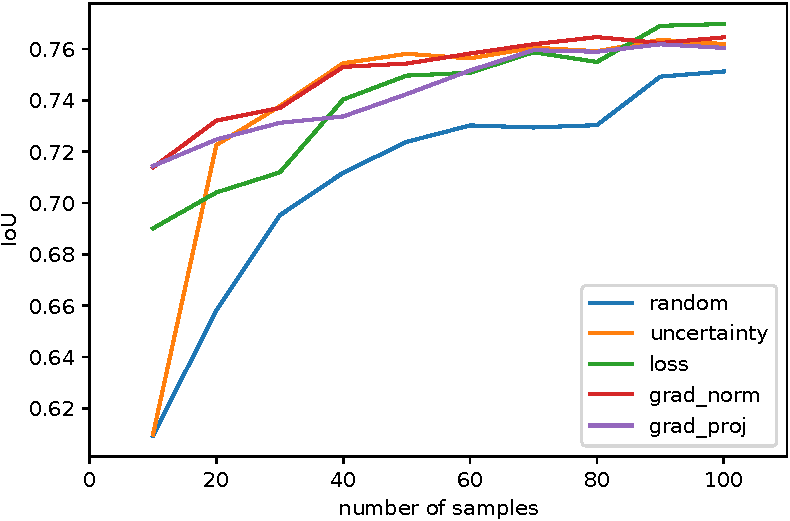
\includegraphics[width=0.8\linewidth]{pics/pw_iou_stuttgart-crop.pdf}
   		\caption{Pixel-wise mean IoU on the Stuttgart dataset. Running the model without any new annotations yields an IoU of $0.34$. Running the model on the whole dataset yields an IoU of 0.79. Gradient-based approaches can reach $90\%$ of the fully supervised performance with 10 samples.}
		\label{fig:iou_stuttgart}    		
%    \vspace{1em}
%   \end{figure}
    \vspace{1.3em}
%   \begin{figure}
    \centering
 %   \vspace{-1em}
    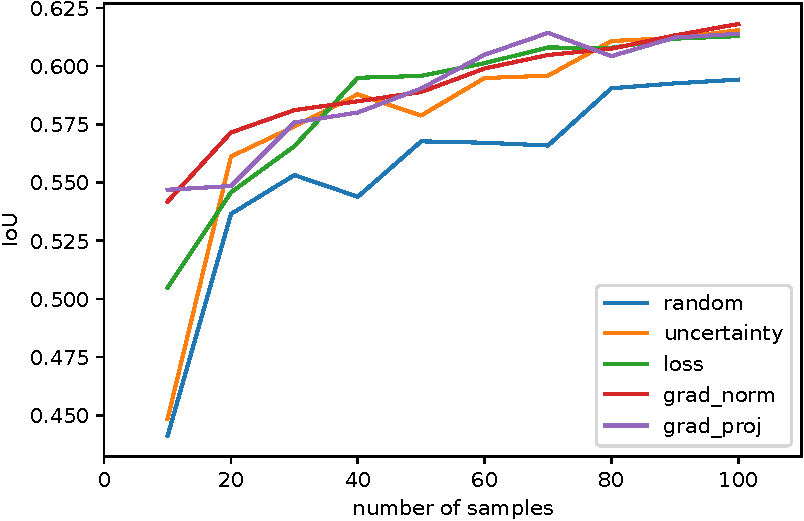
\includegraphics[width=0.8\linewidth]{pics/pw_iou_zurich-crop.pdf}
   		\caption{Pixel-wise mean IoU on the Zurich dataset. Running the model without any new annotations yields an IoU of $0.36$. Running the model on the whole dataset yields an IoU of 0.70. Gradient-based approaches can reach $77\%$ of the fully supervised performance with 10 samples.}
		\label{fig:iou_zurich}    		
 %   \vspace{1em}
   \end{figure}
   
    
Figures \ref{fig:iou_stuttgart} and \ref{fig:iou_zurich} show the performance on the Stuttgart and Zurich datasets when selecting samples for annotation with different methods.  
A few observations can be made: the effect of the sampling method is stronger when only a few images are selected. As the model is trained on more and more samples, the accuracy plateaus as expected and the variation between the different methods decreases. It can be noted however that random sampling has a lower performance even with a greater number of images.

When training the model with only a handful of images, the methods that take into account the impact of the samples on the weights lead to better generalization to the rest of the unseen data. In particular, ranking samples by projecting out gradients results in higher mIoU on both datasets. With 10 samples, which would amount to roughly $1\%$ of the training dataset size, we can achieve $90\%$ of the fully supervised performance (Table~\ref{tab:null_and_fully_supervised}) on the Stuttgart dataset, compared to $76\%$ with random selection. On the Zurich dataset, we can achieve $82\%$ of the fully supervised performance compared to $63\%$ with random selection.


To further quantify the performance of our approach, we use the object-wise metric defined by Milioto \etal~\cite{milioto2018real}, where the accuracy is measured for objects larger than 50 pixels. Since the target application is weeding with agricultural robotics, this metric is more directly useful than pixel-wise performance.  
Table~\ref{tab:object_wise} shows how our approach performs on the Stuttgart and Zurich datasets. Each row shows the mean accuracy when selecting 10 samples with different methods. For comparison, random sampling is shown in the first column. Again, it can be seen that methods measuring the influence of the samples on the weights perform better.


   \begin{table}
 %          \vspace{1em}
        \centering
        \caption{Object-wise Performance on the Stuttgart and Zurich datasets. Each row shows the performance after selecting 10 samples with the different methods and refining the network. Running the model without any new annotations yields an accuracy of $0.15$ on Stuttgart and  $0.33$ on Zurich.}
        \begin{tabular}{@{}cccccc@{}} 
            \toprule
            \makecell{Dataset} & \makecell{Random} & \makecell{Uncertainty} & \makecell{Loss} & \makecell{Gradient \\ Norm} & \makecell{Gradient \\ Proj.} \\ 
            \midrule 
          Stuttgart  & 0.6920 & 0.6437 & 0.7882 & 0.8040 & 0.8196 \\ \addlinespace

          Zurich  & 0.7552 & 0.6943 & 0.7697 & 0.8354 & 0.8025 \\ 
            \bottomrule
        \end{tabular}
        \label{tab:object_wise}
    \end{table}
   


\subsection{Comparision to Other Baselines}
    
To gain more insight into what our baselines are, we ran additional experiments with the results shown in Table~\ref{tab:add_baselines}. 
The first row shows the performance when selecting samples that have the highest entropy:
\begin{align}
e(\bold{x}) &= -\frac{1}{N} \sum_{i=1}^N \sum_{c} p(c \mid x_i) \log p(c \mid x_i),
\end{align}  
\noindent
where $x_i$ is pixel $i$ in image $\bold{x}$, $c$ is the class and $N$ is the number of pixels in the image.

This measure is frequently used in the literature~\cite{chakraborty2015active, zhou2017fine} for active learning. Although it finds samples that the network is uncertain of, it needs to be combined with a measure that provides some diversity in the sample selection. 

%In the second row, we run k-means on the gradients to find clusters that might be representative of the training samples. We found that a number of those clusters had very few samples so a more suitable clustering technique might be needed. 

In the second row, we ran an experiment where we trained the model with the pseudo ground truth first and picked samples randomly afterwards. We found that it performs worse than when picking random samples directly. Although pre-training with the pseudo ground truth allows the network to distinguish foreground vegetation from background, the task at hand is to learn three classes and more importantly distinguish crop from weed. Therefore for all experiments, we refine the model without pre-training on the foreground masks.

In the last row, we run an "oracle" experiment. We find the difference between the parameters of the model without any refinement and the parameters of the fully supervised model. We then find samples with gradients that align with the parameters difference. This experiment is not intended for sample selection, rather to know if the framework had complete knowledge of how the gradients should look like, would it be able to pick better samples. We found that the oracle performance is similar to our gradient-based approaches after seing 10 new samples. This means that \todo{Complete stentence}.

        \begin{table}
           \vspace{1em}
        \centering
        \caption{Additional baselines for training with 10 samples on the Stuttgart dataset. Compare with \figref{fig:iou_stuttgart}.}
        \begin{tabular}{@{}lc@{}} 
            \toprule
            Method  & mIoU \\ 
            \midrule 
             Entropy~\cite{chakraborty2015active, zhou2017fine} & 0.5879   \\ \addlinespace
%    		  K-means  & 0.6396  \\ \addlinespace
    		  Random-pseudo ground truth   & 0.6448  \\ \addlinespace
    		  Align with parameters difference (oracle)  & 0.7010  \\  
            \bottomrule
        \end{tabular}
        \label{tab:add_baselines}
    \end{table}
    
    
    
\subsection{TODO: Find good name}

\todo{Explain with one sentence what this experiment is supposed to show}


\todo{I do not fully understand this and also do not see in the figure the efect of that}
We combined the idea of gradient-based selection with two alternative approaches to achieving diversity in the selected images: Picking on a log scale, or projecting out gradients that have been selected previously. In our experiments, both strategies performed well (]\todo{How do I see that?}). To further analyze them, we plot the t-distributed Stochastic Neighbor Embedding (t-SNE) of the gradients in Figure~\ref{fig:tsne}. Each circle denotes the 2-D embedding of the gradient of a single image before picking the first 10 samples. Samples selected by each method are shown in different colors. We found that both gradient and loss based approaches favor samples that have gradients clustered at the bottom of the plot \todo{What does this mean/imply?}. In our future work we plan to investigate this further.\todo{?}

\todo{It would help to interpret the results and tell the reader what he/she should see.}

 


       \begin{table}
        \vspace{1em}
        \centering
      \caption{Precision and recall on the Stuttgart dataset after selecting the first 10 samples. The first table shows the pixel-wise performance and the second table shows the object-wise performance. The highest values are in bold and the lowest in italics. The uncertainty-based method shows a large imbalance in performance on the two classes.}
        \begin{tabular}{@{}lcccc@{}} 
            \toprule
            & \multicolumn{2}{c}{Precision} & \multicolumn{2}{c}{Recall}\\ 
           \cmidrule{2-5} 
               & Weed & Crop & Weed & Crop \\ 
            \midrule 
    		  Random & \textit{0.4095} & 0.7278 & 0.4851 & \textit{0.6946}  \\ \addlinespace
    		  Uncertainty & 0.5580 & \textit{0.6646} & \textit{0.2711} & \textbf{0.8880}  \\ \addlinespace
    		  Loss & 0.5331 & 0.8025 & 0.6179 & 0.8112  \\ \addlinespace
    		  Gradient Norm & \textbf{0.5970} & 0.8259 & 0.6136 & 0.8402  \\ \addlinespace
    		  Gradient Projection & 0.5745 & \textbf{0.8365} & \textbf{0.6564} & 0.8212  \\ 
            \bottomrule
        \end{tabular}
%        \label{tab:pixel_wise_10_stuttgart}
           ~\\[1mm]
                \begin{tabular}{@{}lcccc@{}} 
            \toprule
            & \multicolumn{2}{c}{Precision} & \multicolumn{2}{c}{Recall}\\ 
           \cmidrule{2-5} 
               & Weed & Crop & Weed & Crop \\ 
            \midrule 
    		  Random & \textit{0.8723} & 0.5740 & 0.6587 & \textit{0.6474}  \\ \addlinespace
    		  Uncertainty & \textbf{0.9476} & \textit{0.4586} & \textit{0.4919} & \textbf{0.8854}  \\ \addlinespace
    		  Loss & 0.9005 & 0.6898 & 0.7811 & 0.7351  \\ \addlinespace
    		  Gradient Norm & 0.9090 & \textbf{0.7390} & 0.7970 & 0.7536  \\ \addlinespace
    		  Gradient Projection & 0.9030 & 0.7308 & \textbf{0.8289} & 0.7375  \\ 
            \bottomrule
        \end{tabular}
 %       \label{tab:object_wise_10_stuttgart}
        \label{tab:performance_10_stuttgart}
    \end{table}
   
    
    
 \begin{figure}
   %  \vspace{-2em} 
    \centering
    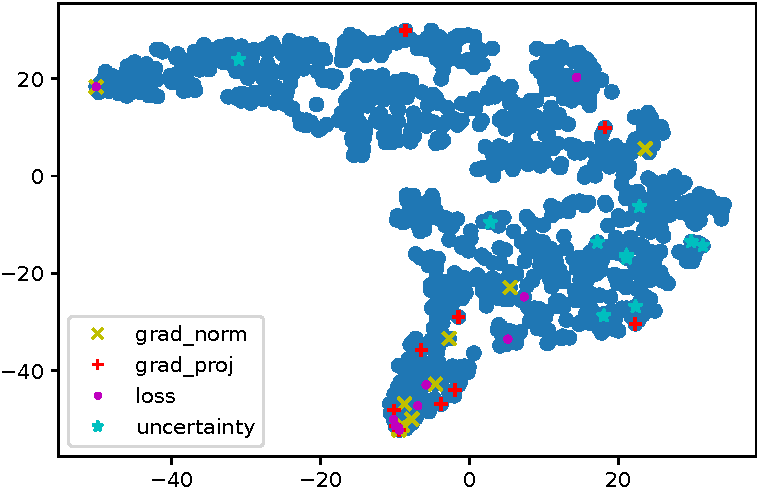
\includegraphics[width=0.8\linewidth]{pics/tsne_all-crop.pdf}
   		\caption{t-SNE of the images gradients on the Stuttgart dataset. Each point represents the 2-D embedding of the gradient vector. The first 10 samples selected by each method are shown in different colors.}
		\label{fig:tsne}    		
  %   \vspace{-1em}
   \end{figure}
   
  
\subsection{Performance on Weed and Crop Classes}
    
A more detailed breakdown of the methods performance is shown in Table~\ref{tab:performance_10_stuttgart}. The first table shows the pixel-wise precision and recall on the Stuttgart dataset after selecting the first 10 samples. Both methods, Gradient Norm and Gradient Projection have a high recall and precision of the crop class without degrading those of the weed class. The object-wise performance in the second table further illustrates the effectiveness of these methods. Gradient Norm and Gradient Projection produce high precision and recall for both classes. The uncertainty-based method, on the other hand, shows a large imbalance of performance on the two classes.
   


%\addtolength{\textheight}{-0.4cm}   % This command serves to balance the column lengths
%                                   % on the last page of the document manually. It shortens
%                                   % the textheight of the last page by a suitable amount.
%                                   % This command does not take effect until the next page
%                                   % so it should come on the page before the last. Make
%                                   % sure that you do not shorten the textheight too much.




%%%%%%%%%%%%%%%%%%%%%%%%%%%%%%%%%%%%%%%%%%%%%%%%%%%%%%%%%%%%%%%%%%%%%%%%%%%%%%%%
\section{Conclusion}
\label{sec:conclusion}

In this paper, we proposed an active learning approach that supports the adaptation
of semantic segmentation networks to  new environments. Our approach  effectively 
selects samples from the new environment for user annotation with the goal of 
minimizing the annotation effort of the user during retraining.
We applied  sample selection strategies to the task crop/weed classification for agricultural robots,
as the appearance between agricultural fields often change substantially such that
re-training is needed. 
In our approach, we compute pseudo ground truth labels using very weakly supervised 
segmentation and use those labels to estimate how new, unlabeled samples will 
affect the weights of the CNN if selected for training. We select the training
samples for user annotation based on the estimated effect on the weights and use them to refine the 
network. Our other ranking methods combine the loss and the uncertainty measures provided by the network with 
log-scale sorting to select samples for annotation.
We evaluated  the performance gain of our gradient-and log based 
approaches on two agricultural  datasets for weed detection. The datasets 
reveal different characteristics from the dataset on which the network was pretrained.
Our results show the effectiveness of our method as it produces higher semantic segmentation
accuracies with a smaller number of training samples, compared to random sampling. As a result
of that, the effort in human annotation is reduced without compromising
performance.
 
     %    \vspace{1em}
%%\bibliographystyle{IEEEtran}
\clearpage
\bibliographystyle{plain}

\bibliography{bibliography}

\end{document}
